Whereas the previous case was concerned with checking the correct implementation and usage of \emph{discrete} fragility functions, the purpose of this case is to verify the correct calculation of damage distribution statistics for a scenario using \emph{continuous} (lognormal CDF) fragility functions.

\begin{table}[htbp]

\centering
\begin{tabular}{ c c c }

\hline
\rowcolor{anti-flashwhite}
\bf{LS} & \bf{Mean IML} & \bf{Std. IML} \\
\hline
\bf{ds1} & 0.50 & 0.40 \\
\bf{ds2} & 1.00 & 0.80 \\
\bf{ds3} & 1.50 & 1.20 \\
\bf{ds4} & 2.00 & 1.60 \\
\hline
\end{tabular}

\caption{Fragility function with zero no damage limit}
\label{tab:ff-cont-tax1-zmin}
\end{table}

Table~\ref{tab:ff-cont-tax1-zmin} shows the mean and standard deviation of the ground motion intensity level for the four damage states, which are the parameters for the lognormal fragility function used in this test case. The fragility model is shown in Figure~\ref{fig:ff-cont-tax1-zmin}.

\begin{figure}[htbp]
\centering
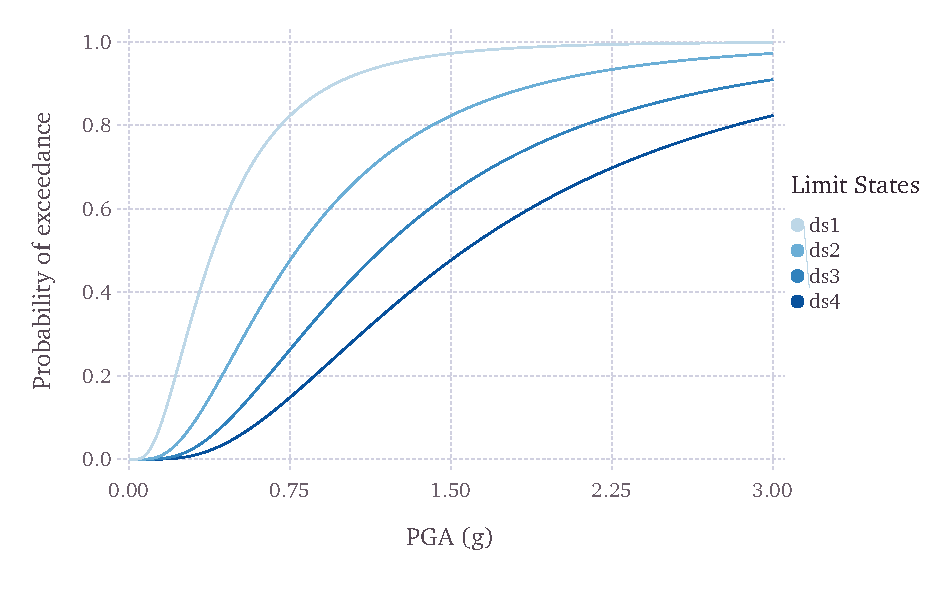
\includegraphics[width=12cm]{qareport/figures/fig-ff-cont-tax1-zmin}
\caption{Continuous (lognormal) fragility model with four damage states}
\label{fig:ff-cont-tax1-zmin}
\end{figure}

The set of five precomputed ground motion values described in Table~\ref{tab:gmfs-diff-l1-5}  are used in this case. The ground motion values at the location of the single asset are $[1.3, 0.044, 0.52, 1.0, 1.2] g$. Consider the first value of $PGA = 1.3 g$. The exceedance probability for damage state $ds_1$ is obtained by employing the equation for the cumulative distribution function for the lognormal distribution, using the mean, $m_1 = 0.5 g$, and standard deviation, $s_1 = 0.4 g$, specified by the fragility function for that damage state. The equations are given below:

\begin{equation}
	\mu_1 = \ln \left( \frac{m_1}{\sqrt{1 + \frac{s_1^2}{m_1^2}}} \right) = -0.940
\end{equation}

\begin{equation}
	\sigma_1 = \sqrt{\ln \left( 1 + \frac{s_1^2}{m_1^2} \right)} = 0.703
\end{equation}

\begin{equation}
	p.o.e.(ds_1) = \frac{1}{2} + \frac{1}{2} erf \left[ \frac{\ln 1.3 - \mu_1}{\sqrt{2} \sigma_1} \right] = 0.956
\end{equation}

Next, the exceedance probabilities for the other damage states for the first ground motion are obtained in a similar manner. We have, for the first ground motion:

\begin{itemize}
	\item $p.o.e.(ds_1) = 0.956$
	\item $p.o.e.(ds_2) = 0.766$
	\item $p.o.e.(ds_3) = 0.559$
	\item $p.o.e.(ds_4) = 0.397$
\end{itemize}

Thus we have exceedance probabilities of $[0.956, 0.766, 0.559, 0.397]$ for $PGA = 1.3 g$. The probabilities of damage state occurrence are given by the pairwise differences of the exceedance probabilities as $[0.956 - 0.766, 0.766 - 0.559, 0.559 - 0.397, 0.397] = [0.190, 0.207, 0.162, 0.397]$. The probability of observing no damage is the remainder of the probability after summing up the probabilities for the four damage states, i.e., $1.0 - (0.190 + 0.207 + 0.162 + 0.397) = 0.044$.

This procedure is repeated for the other four ground motion fields to give the following sets of damage state probabilities:

\begin{itemize}
	\item GMF1: $[0.0436, 0.191, 0.207, 0.162, 0.397]$
	\item GMF2: $[0.9991, 0.0009, 0.000, 0.000, 0.000]$
	\item GMF3: $[0.342, 0.376, 0.157, 0.0652, 0.059]$
	\item GMF4: $[0.091, 0.272, 0.226, 0.148, 0.263]$
	\item GMF5: $[0.055, 0.215, 0.215, 0.160, 0.354]$
\end{itemize}

The mean and standard deviation of the four damage state probabilities and also the probability of observing no damage is now calculated using the above set of probabilities collected from each of the five ground motion simulations.